\subsection{Ellipsoids in a generalized metric space}

%\todo{Georges?}
%\TODO{Smooth out and simplify this description. Add to the plot: unit vectors in data space, and their transformations in canonical space.
%Here it would be useful to describe the geometric relations that pertain to \mat{H}
%(positive semi-definite)
%in the metric of \mat{E} (positive definite).
%I see two sub-figures:
%(a) ellipses for \mat{H} and \mat{E}, showing the conjugate axes and
%bounding parallelogram for \mat{E}, perhaps using the principal component factorization.
%(b) the transformation of (a) using $\mat{H}\mat{E}^{-1}$ or
%$\mat{E}^{-1/2} \, \mat{H} \, \mat{E}^{-1/2}$.
%}

In \appref{sec:conjugate}, we considered the positive semi-definite matrix \mat{W} and
corresponding ellipsoid to be
referred to a Euclidean space, perhaps with different basis vectors.
We showed that various measures of the ``size'' of the ellipsoid could be defined
in terms of functions of the eigenvalues $\lambda_i$ of \mat{W}.

We now consider the generalized
case of an analogous $p \times p$ positive semi-definite symmetric matrix \mat{H}, but where measures of
length, distance, and angles are referred to a metric defined by a positive-definite symmetric
matrix \mat{E}. As is well known, the generalized eigenvalue problem is to find the scalars
$\lambda_i$ and vectors $\vec{v}_i, i=1, 2, \dots p$,
such that $\mat{H} \vec{v} = \lambda \mat{E} \vec{v}$, that is, the roots of
$\det{\mat{H} - \lambda \mat{E}}=0$.

%\TODO{More explanation here ...}
\begin{figure}[htb]
% two figs side-by-side
  \begin{minipage}[c]{.495\textwidth}
   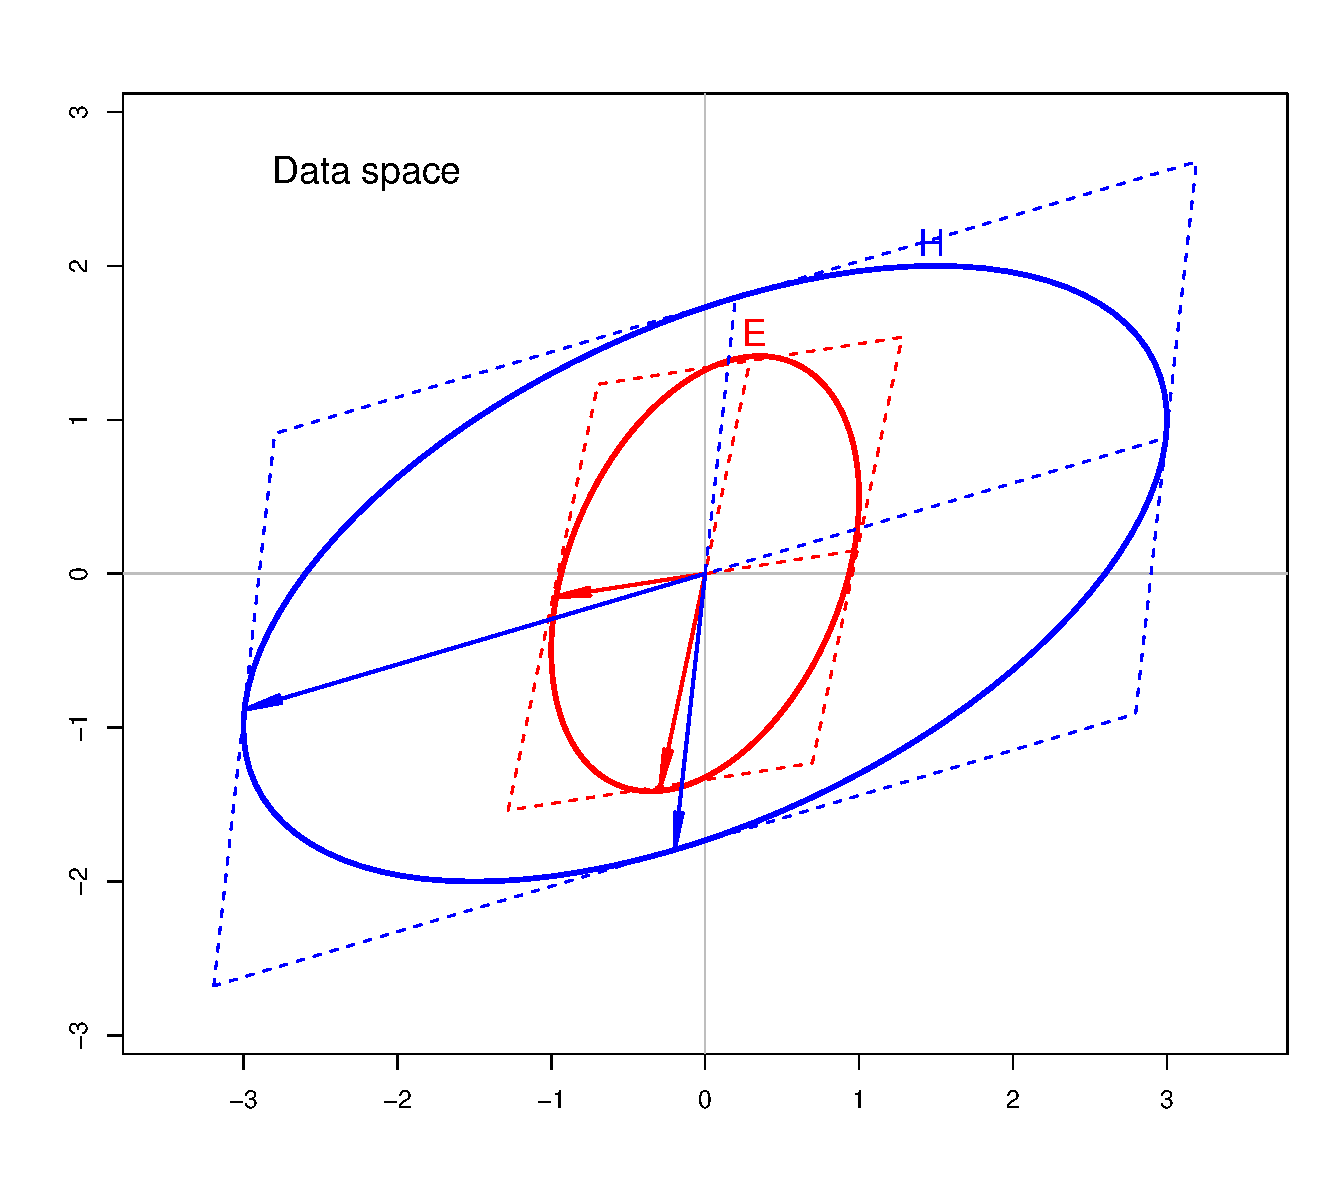
\includegraphics[width=1\linewidth,clip]{fig/ellipse-geneig1}
   \end{minipage}%
  \hfill
  \begin{minipage}[c]{.495\textwidth}
   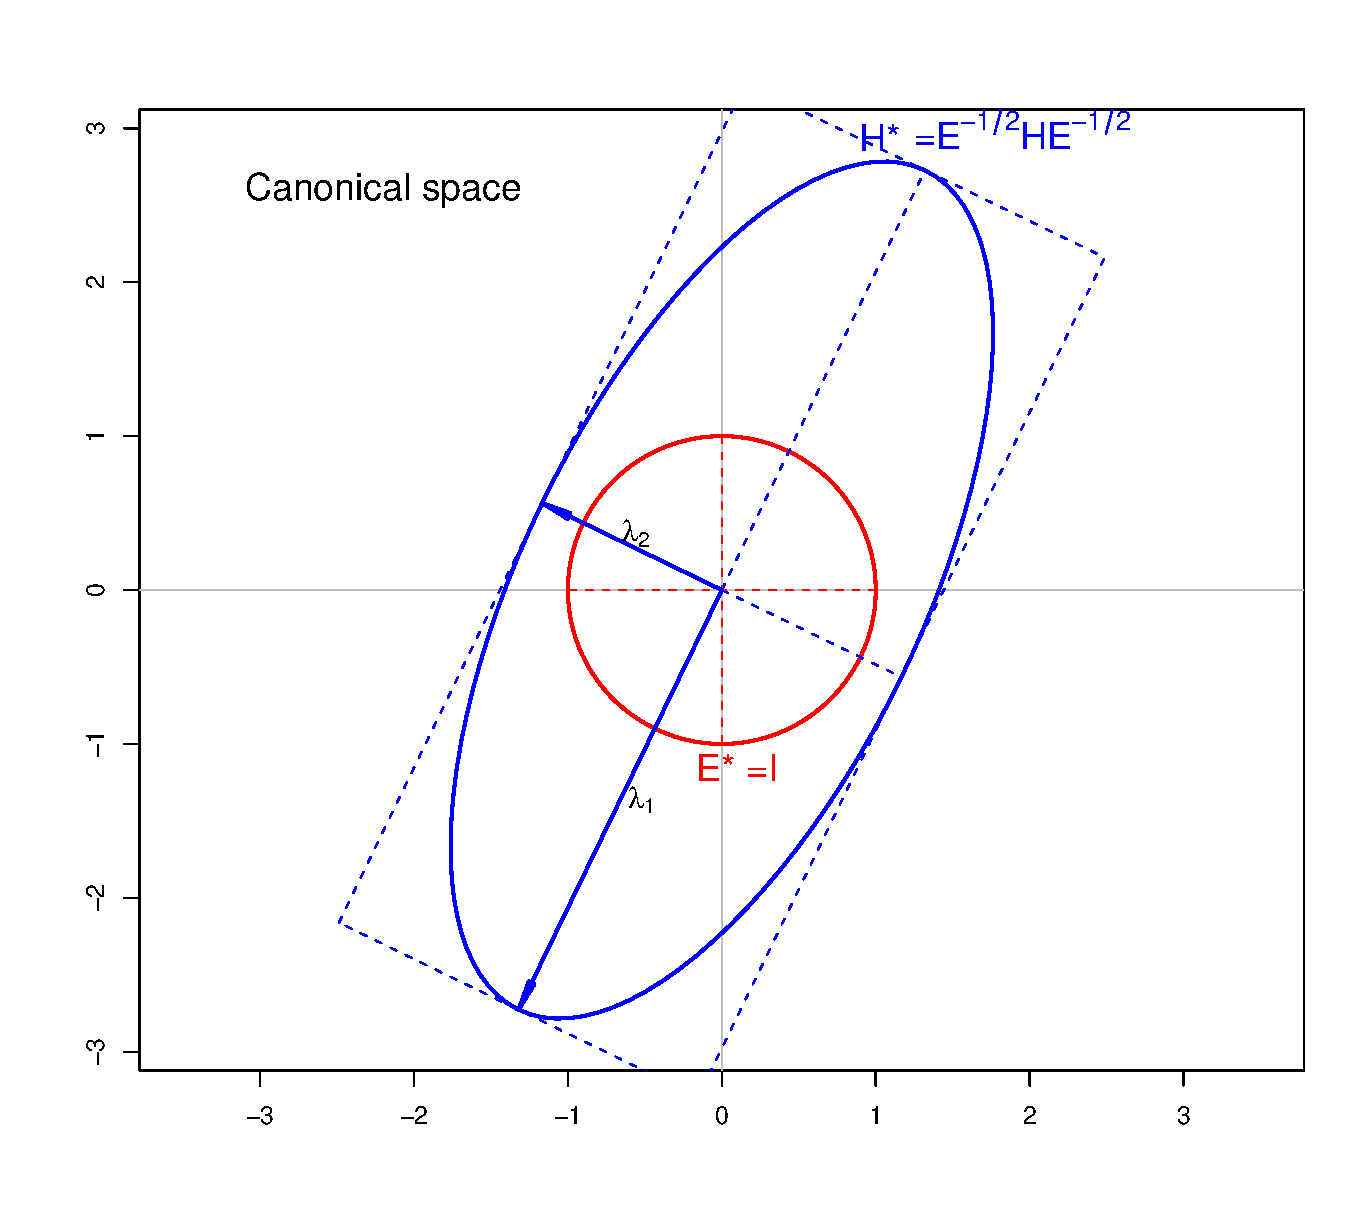
\includegraphics[width=1\linewidth,clip]{fig/ellipse-geneig2}
  \end{minipage}
  \caption{Left: Ellipses for \mat{H} and \mat{E} in Euclidean ``data space.''
   Right: Ellipses for $\mat{H}^\star$ and $\mat{E}^\star$ in the transformed ``canonical space,''
   with the eigenvectors of \mat{H} relative to \mat{E} shown as blue arrows, whose radii
   are the corresponding eigenvalues, $\lambda_1, \lambda_2$. }%
  \label{fig:ellipse-geneig}
\end{figure}
For such \mat{H} and \mat{E}, we can always find a factor \mat{A} of \mat{E}, so that
$\mat{E} = \mat{A} \mat{A}\trans$, whose colums will be conjugate directions for \mat{E}
and whose rows will also be conjugate directions for \mat{H}, in that $\mat{H} = \mat{A}\trans \mat{D} \mat{A}$,
where $\mat{D}$ is diagonal.  Geometrically, this means that there exists a unique pair of
bounding parallelograms for the \mat{H} and \mat{E} ellipsoids whose
corresponding sides are parallel. A linear transformation of \mat{E} and \mat{H}
that transforms the parallelogram
for \mat{E} to a square (or cuboid), and hence \mat{E} to a sphere (or spheroid), generates an
equivalent view in what we describe below as canonical space.


In statistical applications (e.g., MANOVA, canonical correlation), the generalized
eigenvalue problem is transformed to an ordinary eigenvalue problem by considering
the following equivalent forms with the same $\lambda_i$, $\vec{v}_i$,
\begin{eqnarray*}
(\mat{H} - \lambda \mat{E}) \vec{v} & = & \vec{0} \\
\Rightarrow (\mat{H} \, \inv{\mat{E}} - \lambda \mat{I}) \vec{v} & = & \vec{0} \\
\Rightarrow (\invhalf{\mat{E}} \, \mat{H} \, \invhalf{\mat{E}} - \lambda \mat{I}) \vec{v} & = & \vec{0} \comma
\end{eqnarray*}
where the last form gives a symmetric matrix, $\mat{H}^\star = \invhalf{E} \, \mat{H} \, \invhalf{E}$.
Using the square root of \mat{E} defined by the
principal-component factorization $\half{E} = \mat{\Gamma} \half{\mat{\Lambda}}$ produces
the ellipsoid  $\mat{H}^\star$, the
orthogonal axes of which correspond to the $\vec{v}_i$, whose squared radii are the corresponding %% squared / GM
eigenvalues $\lambda_i$.  This can be seen geometrically as a rotation of ``data space''
to an orientation defined by the principal axes of \mat{E}, followed by a re-scaling, so
that the \mat{E} ellipsoid becomes the unit spheroid.  In this transformed space
(``canonical space''), functions of the
the squared radii $\lambda_i$ of the axes of $\mat{H}^\star$ give direct measures of %% squared / GM
the ``size'' of \mat{H} relative to \mat{E}. The orientation of the eigenvectors
$\vec{v}_i$ can be related to the (orthogonal) linear combinations of the
data variables that are successively largest in the metric of \mat{E}.


To illustrate, \figref{fig:ellipse-geneig} (left) shows
the ellipses generated by
\begin{equation*}
 \mat{H} = \left[ \begin{array}{cc}
                   9 & 3 \\
                   3 & 4
                  \end{array}\right]
 \quad \mbox{ and } \quad
 \mat{E} = \left[ \begin{array}{cc}
                   1 & 0.5 \\
                   0.5 & 2
                  \end{array}\right]
\end{equation*}
together with their conjugate axes. For \mat{E}, the conjugate axes are defined by the columns of the right factor,
$\mat{A}\trans$,
in $\mat{E} = \mat{A} \mat{A}\trans$; for \mat{H}, the conjugate axes are defined by the columns of $\mat{A}$.
The transformation to $\mat{H}^\star = \invhalf{E} \, \mat{H} \, \invhalf{E}$ is shown in the right panel
of \figref{fig:ellipse-geneig}. In this ``canonical space,'' angles and lengths have the orginary interpretation
of Euclidean space, so the size of $\mat{H}^\star$ can be interpreted directly in terms of functions of
the radii $\sqrt{\lambda_1}$ and $\sqrt{\lambda_2}$.

